\section{Metodologia}

\subsection{Modulação AM-DSB-SC (Double Sideband Suppressed Carrier)}

Neste experimento foi utilizado o GNU Radio Companion (GRC) para implementar a modulação AM-DSB-SC. O sinal de mensagem foi gerado utilizando um bloco de fonte de sinal senoidal, com frequência fm de 1kHz e amplitude de 1. A portadora foi gerada com uma frequência de 5kHz e amplitude de 1. O sinal modulado foi obtido multiplicando o sinal de mensagem pela portadora.

O diagrama de blocos da modulação AM-DSB-SC no GNU Radui é apresentado na Figura \ref{fig:modulacao_am_sc}
\begin{figure}
    \centering
    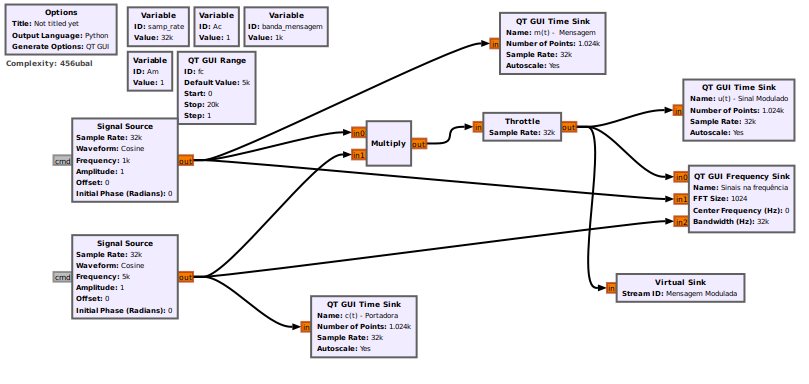
\includegraphics[width=0.5\textwidth]{images/modulacao_gnu_am_dsb_sc.png}
    \caption{Diagrama de blocos da modulação AM-DSB-SC. Fonte: Autor.}
    \label{fig:modulacao_am_sc}
\end{figure}

Os seguintes blocos foram utilizados:

\begin{itemize}
    \item \textbf{Signal Source}: Gera o sinal de mensagem com frequência de 1000 Hz e amplitude de 1 .
    \item \textbf{Signal Source}: Gera a portadora com frequência de 0 à 20kHz,e amplitude de 1 V.
    \item \textbf{Signal Source}: Gera o oscilador local com frequência fixa de 5kHz.
    \item \textbf{QT GUI Range}: Permite ajustar a frequência da portadora. Aqui foi denido entre 0 e 20kHz.
    \item \textbf{Multiply}: Multiplica o sinal de mensagem pela portadora, resultando no sinal modulado AM-DSB-SC.
    \item \textbf{Virtual Sink}: Permite armazenar o sinais e usalos no bloco Virtual Source.
    \item \textbf{Virtual Source}: Permite usar os sinais armazenados no bloco Virtual Sink.
    \item \textbf{QT GUI Time Sink}: Exibe o sinal modulado no domínio do tempo.
    \item \textbf{QT GUI Frequency Sink}: Exibe o espectro do sinal modulado no domínio da frequência.
\end{itemize}


Para mostrar a perda da mensagem pela falta de sincronismo, foi ajustado a frequência da portadora para uma frequência de 10Khz.

\subsection{Demodulação AM-DSB-SC (Double Sideband Suppressed Carrier)}

De maneira semelhante, foi implementada a demodulação do sinal AM-DSB-SC utilizando o GNU Radio Companion. O sinal modulado foi multiplicado novamente por um sinal da portadora (oscilador local) com a mesma frequência e fase da portadora original, seguido de um filtro passa-baixas para recuperar o sinal de mensagem.

O diagrama de blocos da demodulação AM-DSB-SC no GNU Radio é apresentado na Figura \ref{fig:demodulacao_am_sc_gnu}.

\begin{figure}
    \centering
    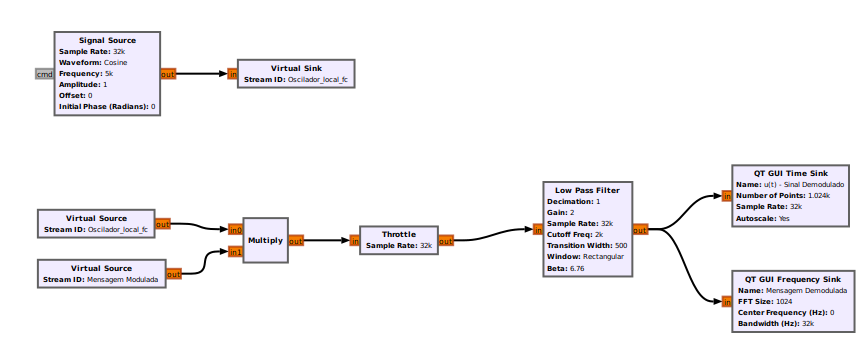
\includegraphics[width=0.5\textwidth]{images/demodulacao_gnu_am_dscb_sc.png}
    \caption{Diagrama de blocos da demodulação AM-DSB-SC. Fonte: Autor.}
    \label{fig:demodulacao_am_sc_gnu}
\end{figure}

Os seguintes blocos foram utilizados:

\begin{itemize}
    \item \textbf{Virtual Source}: Recebe o sinal modulado armazenado anteriormente.
    \item \textbf{Signal Source}: Gera o oscilador local com frequência igual à portadora (5kHz).
    \item \textbf{Multiply}: Multiplica o sinal modulado pelo oscilador local.
    \item \textbf{Throtle}: Controla a taxa de amostragem do fluxo de dados, evitando sobrecarga do processamento durante a simulação.
    \item \textbf{Low Pass Filter}: Frequencia de corte em 2kHz, com ganho de 2 e a janela na forma retangular.
    \item \textbf{QT GUI Time Sink}: Exibe o sinal demodulado no domínio do tempo.
    \item \textbf{QT GUI Frequency Sink}: Exibe o espectro do sinal demodulado no domínio da frequência.
\end{itemize}

Para demonstrar a importância do sincronismo, foi realizada a demodulação com o oscilador local defasado ou com frequência diferente, observando a distorção ou perda do sinal de mensagem.

